\documentclass[11pt]{article}
\usepackage[margin=1in]{geometry}
\usepackage{amsmath,amssymb}
\usepackage{booktabs}
\usepackage{tikz}
\usetikzlibrary{shapes.geometric,arrows.meta,positioning}
\usepackage{pgfplots}
\pgfplotsset{compat=1.9}
\usepackage[colorlinks=true,linkcolor=blue,citecolor=blue,urlcolor=blue]{hyperref}

\title{A Receipt-First Estate: Honest Operational Accounting of a Governed AI Research Organization\\ \large November 2026 Census Edition}
\author{Stephen P.\ Lutar Jr.\\ SZL Holdings, Inc.\\ \texttt{ORCID 0009-0001-0110-4173}}
\date{November 15, 2026}

\begin{document}
\maketitle

\begin{abstract}
This report is an operational accounting of a governed AI research estate --- the SZL Holdings organization --- written under a receipt-first doctrine in which every measured claim is bound to a dated, addressable artifact (a repository commit, an API-observable receipt file, or a DOI-minted record), and every unmeasured claim is labeled as such. The estate comprises a GitHub organization of 159 repositories, a Hugging Face organization whose public face on the census date exposes 131 models, 71 datasets, and 32 Spaces through the anonymous API, a Lean~4/Mathlib proof corpus with a locked registry of exactly eight machine-checked formulas, and an on-chain receipt substrate exceeding one thousand receipt files. We report: (i) continuous-integration health of 121 of 130 active repositories green at last run; (ii) a full-corpus proof-attempt campaign of 143/143 attempts with 65 honestly recorded \texttt{sorry}-echo failures and zero fabrications; (iii) an evaluation battery whose most recent binding wave scores 37 of 41 bindings at 0/6 with disclosed abstention failures --- reported as the headline finding it is, not smoothed; (iv) receipt-gated corpus admission measured at 2.67\%, 1.33\%, 20.67\%, and 21.90\% across four gates with per-row denominators published; and (v) a disclosed incident in which a marketing-stamping job overwrote 138 public model cards and was repaired by byte-exact, commit-addressed restoration. Every figure in this paper is generated from data read on November 14--15, 2026, from live APIs or on-disk logs, and the provenance of each figure is tabulated in the appendix. The paper claims operational honesty, not scientific novelty: no benchmark here is state-of-the-art, several measured results are failures, and the contribution is the accounting discipline itself.
\end{abstract}

\section{Introduction and Doctrine}
\label{sec:intro}

Agentic AI organizations face an accounting problem before they face a science problem. When a research estate produces models, datasets, proofs, deployments, and publications at machine speed, the binding constraint on trust is not the production rate but the \emph{verifiability rate}: the fraction of claims whose evidence can be re-read by a third party at a stable address. This report describes an estate built around one constraint: \textbf{no claim without a receipt}.

The doctrine has three tiers, applied uniformly:
\begin{itemize}
\item \textbf{MEASURED}: a dated artifact (receipt file, API record, CI run) at a stable address backs the claim.
\item \textbf{UNKNOWN}: no artifact exists; the claim is explicitly not made.
\item \textbf{ABSTAIN}: an artifact exists and records a failure or a refusal to answer; the failure is published as a first-class result.
\end{itemize}

The tiers exist because the failure mode of agentic research organizations is not lying but \emph{drift}: a claim that was once measured survives into contexts where its measurement no longer applies, and a card that was once honest accumulates language faster than evidence. A three-tier discipline makes drift detectable --- an unmeasured claim is not merely weak, it is \emph{noncompliant} with the estate's own published standard, and any reader can cite the tier against it. The tiers also price honesty correctly: ABSTAIN results cost publication prestige but buy the only currency that compounds --- a reader who has seen the estate publish its failures has a reason to believe its successes.

Under this doctrine a 0/6 evaluation score is not an embarrassment to be buried; it is a receipt. Section~\ref{sec:battery} reports exactly such a wave. The estate's public interfaces are: the GitHub organization \texttt{szl-holdings} (159 repositories), the Hugging Face organization \texttt{SZLHOLDINGS} (public census in Section~\ref{sec:census}), the Lean~4 proof corpus at the frozen repository \texttt{szl-holdings/lutar-lean}, and the receipt datasets described in Section~\ref{sec:substrate}. Two companion papers --- one on machine-checked append-only governance (25 pages) and one on a graph-shaped audit of governance aggregation (26 pages) --- carry the formal content; this report is the operational layer beneath them: what exists, what is green, what failed, and where every number lives.

\paragraph{Scope and honesty boundary.} This is not a survey of scientific results. It is an operational census. Numbers are point-in-time (November 14--15, 2026), API-observable, and reproducible by the commands in Section~\ref{sec:repro}. Where the estate failed, the failure is printed with the same typography as the successes.

\paragraph{How to read this paper.} Sections~\ref{sec:census}--~\ref{sec:lean} are the census layer: what exists and how healthy it is. Sections~\ref{sec:tracka}--~\ref{sec:battery} are the measurement layer: the two flagship honesty instruments, both reported with their failures exposed. Sections~\ref{sec:cards}--~\ref{sec:deploy} are the case-study layer: integrity, delivery, and a gate series with per-row denominators. Section~\ref{sec:incident} is the incident record at full length. Sections~\ref{sec:loop}--~\ref{sec:change} are the operating layer, and Sections~\ref{sec:limits}--~\ref{sec:concl} state what the paper does not claim. A reader with ten minutes should read the abstract, Figure~\ref{fig:battery}, Table~\ref{tab:gates}, and Section~\ref{sec:incident}; the rest is the audit trail.

\section{Estate Census}
\label{sec:census}

\subsection{GitHub organization}
The GitHub organization \texttt{szl-holdings} holds \textbf{159 repositories} (25 private, 29 archived at census time). The active-repo language profile is dominated by Python, with TypeScript, HTML/JS, Lean (\texttt{lutar-lean}), TeX (\texttt{szl-papers}), and CSS as secondary families. The two paper-bearing repositories are \texttt{szl-papers} (LaTeX sources, preprint metadata, DOI registry) and \texttt{lutar-lean} (Lean~4/Mathlib proof corpus and its attempt receipts). The repositories of record referenced throughout this paper are listed in Table~\ref{tab:repos}.

\begin{table}[htbp]
\centering
\small
\begin{tabular}{lp{8.8cm}}
\toprule
\textbf{Repository} & \textbf{Role} \\
\midrule
\texttt{szl-papers} & Paper sources, preprint metadata, DOI registry (this report included). \\
\texttt{lutar-lean} & Lean~4/Mathlib proof corpus, locked registry, attempt receipts. \\
\texttt{szl-forge} & Delivery pipeline: model-card governance, publisher workflows, CI frontier checks. \\
\texttt{a11oy} & Live estate application; main HEAD mirrored by the honest-status endpoint. \\
\texttt{szl-safe-stack} & Safety-stack components (carries the disclosed CI deadlock of \S\ref{sec:ci}). \\
\texttt{platform} & Estate platform services. \\
\texttt{szl-org-health} & Organization health automation (merge receipts of \S\ref{sec:change}). \\
\texttt{SZLHOLDINGS/frontier-54-runs} & Receipt substrate dataset (\S\ref{sec:substrate}). \\
\texttt{SZLHOLDINGS/lean-proof-corpus-v1} & Proof-corpus dataset with the 143 Track A attempt receipts. \\
\bottomrule
\end{tabular}
\caption{Repositories of record for this census. Every figure in this paper reads from one of these addresses.}
\label{tab:repos}
\end{table}

\subsection{Hugging Face organization}
The anonymous public API on the census date returns:
\begin{center}
\begin{tabular}{lrl}
\toprule
\textbf{Artifact} & \textbf{Public count} & \textbf{Endpoint} \\
\midrule
Models & 131 & \texttt{/api/models?author=SZLHOLDINGS} \\
Datasets & 71 & \texttt{/api/datasets?author=SZLHOLDINGS} \\
Spaces & 32 & \texttt{/api/spaces?author=SZLHOLDINGS} \\
\bottomrule
\end{tabular}
\end{center}
The 32 public Spaces include the estate's live application surfaces --- the showcase, the estate's primary Space, and the organization card --- which the probe sweep of Section~\ref{sec:edge} returns HTTP 200 for. These are \emph{anonymous} counts: privately held repositories (45 models at the November 14 audit) are not visible to the unauthenticated endpoint and are excluded here rather than estimated. An earlier authenticated audit recorded 183 model repositories including private ones; that figure is not re-claimed here because the census instruments differ. The private vault (45 model repositories at the November 14 audit) is composed of laptop-LoRA mirrors, enterprise candidates, organization placeholders, and triage-stage candidates; exposure is contained by privacy, and the same fail-closed card rules govern it --- the audit found all 45 carried the same wave-4 stamp signature and none is claimed as measured here. Figure~\ref{fig:census} shows the public census.

\begin{figure}[htbp]
\centering
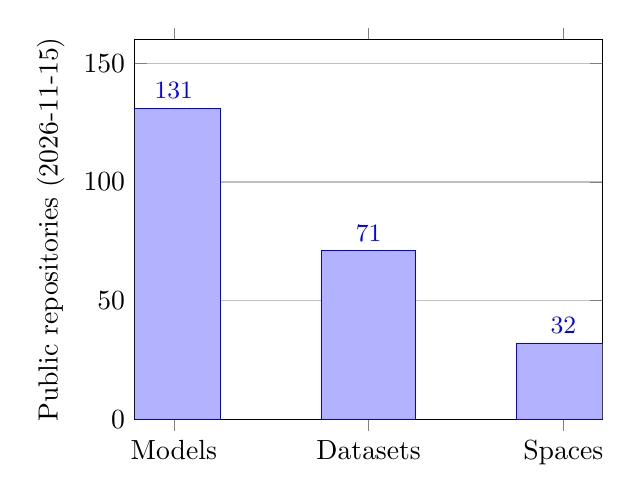
\begin{tikzpicture}
\begin{axis}[
  ybar, bar width=34pt,
  width=0.62\textwidth, height=6.4cm,
  symbolic x coords={Models, Datasets, Spaces},
  xtick=data, ymin=0, ymax=160,
  ylabel={Public repositories (2026-11-15)},
  nodes near coords, every node near coord/.append style={font=\small},
  ymajorgrids=true,
]
\addplot coordinates {(Models,131) (Datasets,71) (Spaces,32)};
\end{axis}
\end{tikzpicture}
\caption{Public Hugging Face census, anonymous API, November 15, 2026. Private repositories are excluded by instrument, not by choice.}
\label{fig:census}
\end{figure}

\subsection{The vertical map}
The estate is organized as twelve research verticals. Figure~\ref{fig:verticals} maps them with their census status. Each vertical's claims live in its own repositories and receipt namespaces; none of the twelve is claimed to be complete, and two (Clinical/Transport Observability, Creativity) are explicitly early-stage with artifact-honest cards only.

\begin{figure}[htbp]
\centering
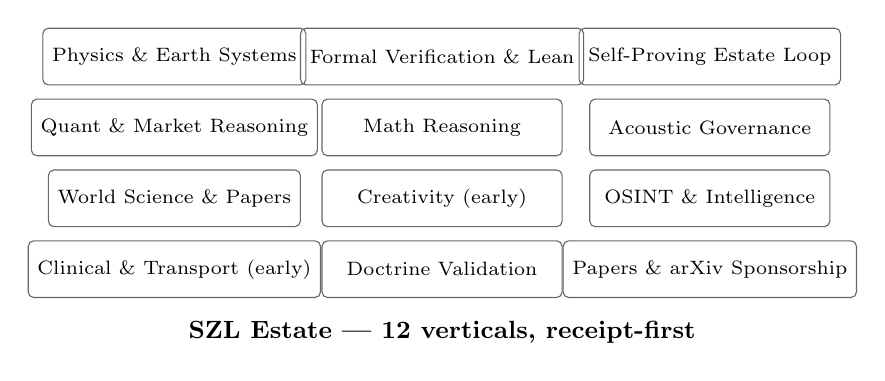
\begin{tikzpicture}[
  box/.style={draw=black!60, rounded corners=2pt, align=center, font=\scriptsize, minimum width=3.05cm, minimum height=0.72cm},
]
\node[box] (p) at (0,3.0) {Physics \& Earth Systems};
\node[box] (l) at (3.4,3.0) {Formal Verification \& Lean};
\node[box] (s) at (6.8,3.0) {Self-Proving Estate Loop};
\node[box] (q) at (0,2.1) {Quant \& Market Reasoning};
\node[box] (m) at (3.4,2.1) {Math Reasoning};
\node[box] (a) at (6.8,2.1) {Acoustic Governance};
\node[box] (w) at (0,1.2) {World Science \& Papers};
\node[box] (c) at (3.4,1.2) {Creativity (early)};
\node[box] (o) at (6.8,1.2) {OSINT \& Intelligence};
\node[box] (t) at (0,0.3) {Clinical \& Transport (early)};
\node[box] (d) at (3.4,0.3) {Doctrine Validation};
\node[box] (x) at (6.8,0.3) {Papers \& arXiv Sponsorship};
\node[draw=none, font=\small\bfseries] at (3.4,-0.5) {SZL Estate --- 12 verticals, receipt-first};
\end{tikzpicture}
\caption{The twelve-vertical estate map as tracked on the internal frontier board. Two verticals are marked early-stage; no vertical is claimed complete.}
\label{fig:verticals}
\end{figure}
